\section{Cytologie}

\subsection{Basics}

	\begin{itemize}
		\item Domänen: Bacteria, Archaea und Eukarya
	\end{itemize}

\subsection{Aufbau}

	\begin{figure}[ht!]
	\leavevmode
	\begin{center}
	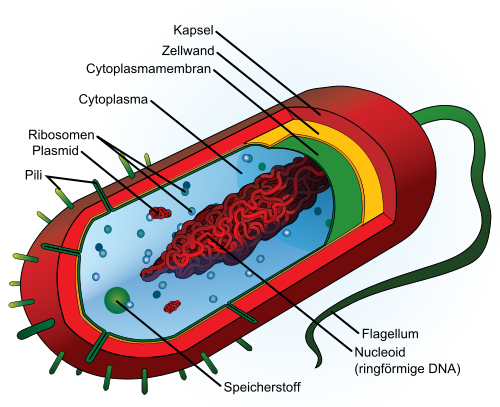
\includegraphics[scale=0.47]{./pictures/avg_prokaryote_cell_500}
	\end{center}
	\caption{\slshape{Typische prokaryotische Zelle.}}
	\label{fig:prokarya}
	\end{figure}

	\begin{figure}[ht!]
	\leavevmode
	\begin{center}
	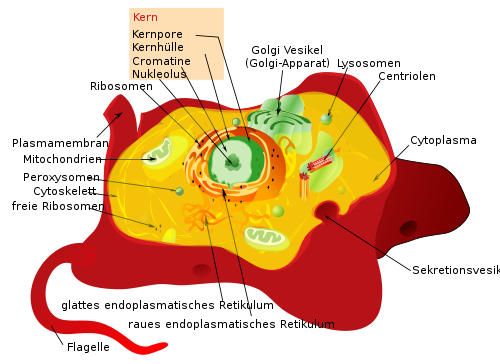
\includegraphics[scale=0.47]{./pictures/animal_cell_500}
	\end{center}
	\caption{\slshape{Tierische Zelle als Beispiel einer eukaryotischen Zelle.}}
	\label{fig:eukarya}
	\end{figure}


\subsection{Membran}

\subsection{Zellwand}
